\documentclass{abgabe}
\usepackage{standalone}

\usepackage{listings}
\usepackage{xcolor}
\usepackage{newtxtt}

\definecolor{darkviolet}{rgb}{0.5,0,0.4}
\definecolor{darkgreen}{rgb}{0,0.4,0.2}
\definecolor{darkblue}{rgb}{0.1,0.1,0.9}
\definecolor{darkgrey}{rgb}{0.5,0.5,0.5}
\definecolor{lightblue}{rgb}{0.4,0.4,1}

\lstset{
    language=Java,
    basicstyle=\small\ttfamily,
    keywordstyle=\color{darkviolet}\bfseries,
    commentstyle=\color{darkgreen},
    stringstyle=\color{darkblue},
    morecomment=[s][\color{lightblue}]{/**}{*/},
    showstringspaces=false,
    frame = single,
    %numbers=left
    }
    
\setauthor{Patrick Gustav Blaneck} % Autor hier
\setmodule{Softwaretechnik} % Modulname hier
%\setmodule{Buzzword-Bingo} % Modulname hier
\setsheetnum{9} % Blattnummer hier
%\setsheettype{Übungsblatt} % Blatttyp hier

\begin{document}
\maketitle
\begin{questions}
    \begingroup
    \renewenvironment{questions}{}{}
    %\setcounter{question}{5}
    
\documentclass{abgabe}
\begin{document}

\begin{questions}
    \qformat{\thequestion. \textbf{\thequestiontitle} \hfill}
    \titledquestion{Veranstaltungsverwaltungssystem}

    Gegeben sei folgende Beschreibung für ein Veranstaltungsverwaltungssystem:

    Personen haben Zeichenketten als Name.
    Studenten sind Personen, erben also die Eigenschaften von Person, haben aber zusätzlich eine ganzzahlige Matrikelnummer und nehmen an beliebig vielen Veranstaltungen teil.
    Eine Veranstaltung hat potentiell beliebig viele Teilnehmer, wird aber von einem, zwei oder drei Mitarbeitern betreut.
    Eine Veranstaltung hat eine Veranstaltungsnummer und einen Titel.
    Seminare und Vorlesungen sind spezielle Veranstaltungen.
    Ein Seminar hat eine begrenzte Anzahl an Plätzen, für eine Vorlesung wird eine Klausur angeboten oder nicht.
    Mitarbeiter sind Personen und betreuen eine bis fünf Veranstaltungen und haben eine Personalnummer.
    Professoren und Assistenten sind Mitarbeiter.
    Assistenten sind bei genau einem Professor beschäftigt und haben eine bestimmt Finanzierung (Zeichenkette).
    Ein Professor hat ein Lehrgebiet (Zeichenkette), beschäftigt beliebig viele Assistenten und ist Inhaber von genau einem Lehrstuhl.
    Ein Lehrstuhl hat eine Bezeichnung und genau einen Professor als Inhaber.

    Erstellen Sie anhand der obigen Beschreibung ein \emph{Klassendiagramm}.
    Ihr Diagramm sollte folgende Punkte beinhalten:
    \begin{itemize}
        \item \emph{Generalisierungsbeziehungen},
        \item \emph{Assoziationen} mit Assoziationsnamen und Leserichtung,
        \item \emph{Multiplizitäten} sowie
        \item \emph{Attributnamen} und (sinnvolle) \emph{–typen}.
    \end{itemize}

    Finden Sie jeweils ein Beispiel, bei dem eine Aggregations- und eine Kompositionsbeziehung sinnvoll ist.
    Erläutern Sie kurz den Unterschied zwischen Aggretation und Komposition anhand des Bespiels.
    \newpage 
    \begin{solution}
        \begin{center}
            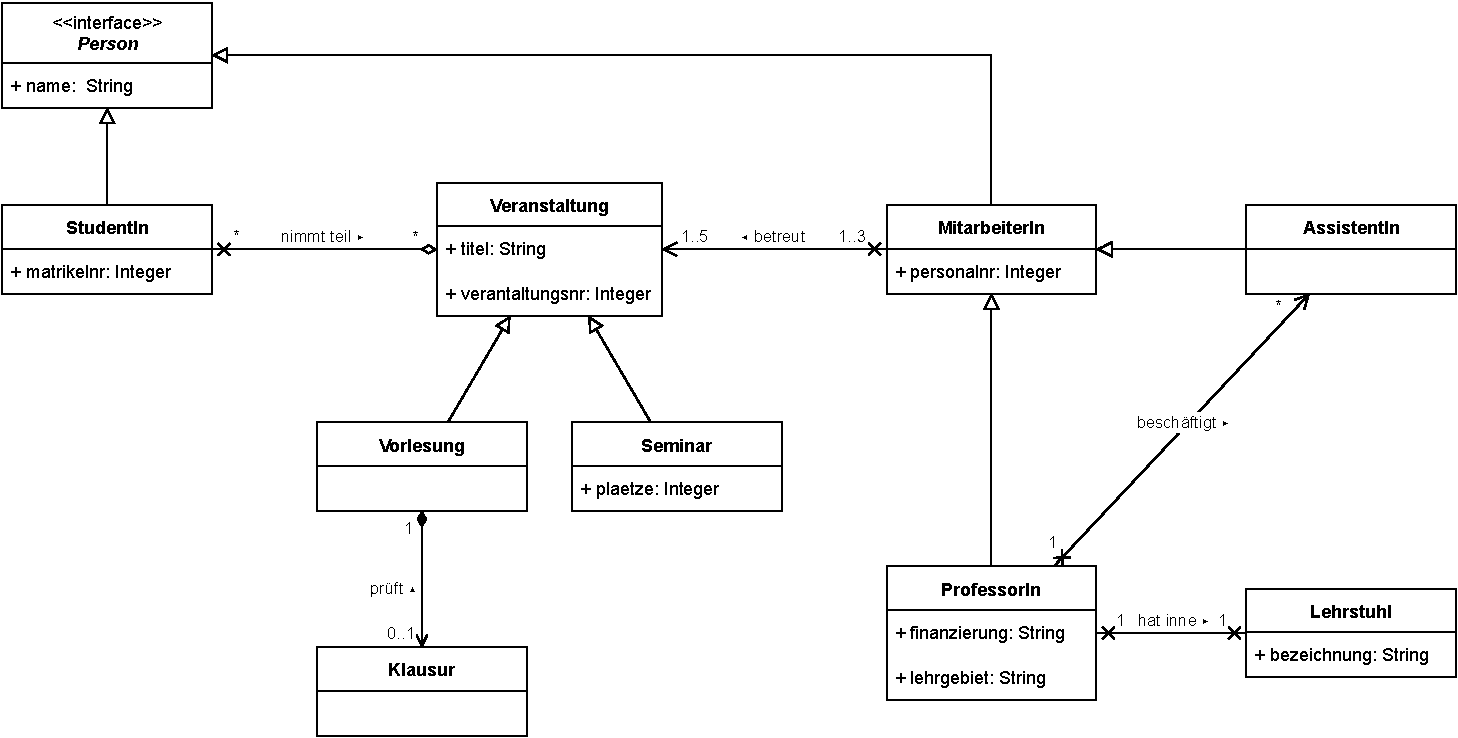
\includegraphics[width=\textwidth]{swt_h07_veranstaltungsverwaltung.pdf}
        \end{center}

        Reddit=User \href{https://www.reddit.com/r/javahelp/comments/gpnqij/comment/frnuudx/?utm_source=share&utm_medium=web2x&context=3}{raja\_42} fasst den Unterschied zwischen Aggregation und Komposition gut zusammen:
        \begin{displayquote}
            Association is a relationship between two entities. Kind of, associated with, in English.

E.g. An Employee class will have a property which is a list of Projects.

Composition is when a container entity has child entities which cannot survive on their own.

E.g. A Shopping Cart class is composed of a list of Cart Items. When a Shopping Cart is deleted, the Cart Items cannot exist conceptually. So they are transient in nature.

Any physical representation of them in database etc. will follow this principle. E.g. There will never be a Cart Item record in the DB without a Shopping Cart record id.

Finally, an aggregation is like composition except the contained entities can exist on their own.

E.g. When you are selecting a group of people in a classroom for a science project, you model few entities or classes.

A Student class for every student in the class. A Professor entity. Etc.

A ProjectGroup class is an aggregation which then has a list of students, a professor etc.

Both are independent concepts. Dissolving a project group doesn't make the corresponding students and professors vanish from the system. They still exist.

In physical form, they represent DB records that don't get deleted when the container record is deleted. This just means that they are independent entities that can live on their own.
        \end{displayquote}
    \end{solution}
\end{questions}
\end{document}
    \newpage
    
\documentclass{abgabe}
\begin{document}

\begin{questions}
    \qformat{\thequestion. \textbf{\thequestiontitle} \hfill}
    \titledquestion{Veränderte Anforderungen}
    Einem Kunden fällt nach Zweidritteln erfolgreicher Projektlaufzeit ein, dass er eine bereits entwickelte Funktionalität nicht benötigt, dafür aber eine andere wünscht. 
    Beschreiben Sie kurz, wie man bei Nutzung der folgenden Vorgehensmodelle darauf reagieren würde:
    \begin{parts}
        \part 
        Wasserfallmodell
        \begin{solution}
            \begin{center}
                
\includegraphics[width=0.5\textwidth]{crying.png}
            \end{center}
            
            Und Erklärung:
            
            Wenn man erst einmal davon absieht, dass das Wasserfall-Modell nach Royce bewiesenermaßen \href{http://valueatwork.se/waterfall-model-probably-the-most-costly-mistake-in-the-world/?lang=en}{ohnehin nicht funktioniert}, sieht das Wasserfallmodell keine Möglichkeit der Reevaluation vor. 
            Ergo wird bei striktem Ablauf nach dem Wasserfallmodell die Anforderung einfach ignoriert.
        \end{solution}
        
        \part 
        Iterative Entwicklung
        \begin{solution}
            Man kann hoffen, dass die zu verändernde Funktionalität nicht zu viele Änderungen am bisher entwickelten System hervorruft. 
            Ist dies der Fall, kann man in der nächsten Iteration die benötigten Änderungen vornehmen.
            
            Sind allerdings zu viele Änderungen nötig, muss potentiell die gesamte Codebase verändert oder neugebaut werden. 
            Das kann entweder einen (quasi) Neustart, oder das gleiche Ergebnis wie in (a) hervorrufen.
        \end{solution}
        
        \part 
        Inkrementelle Entwicklung
        \begin{solution}
            Man kann hoffen, dass das zu verändernde Inkrement nicht zu viele Änderungen am bisher entwickelten System hervorruft. 
            Ist dies der Fall, kann man in dem nächsten Inkrement die benötigten Änderungen vornehmen.
            
            Sind allerdings zu viele Änderungen nötig, muss potentiell die gesamte Codebase verändert oder neugebaut werden. 
            Das kann entweder einen (quasi) Neustart, oder das gleiche Ergebnis wie in (a) hervorrufen.
        \end{solution}
        
        \newpage
        \part 
        Wo würden Sie das SCRUM Modell einordnen?
        \begin{solution}
            Aus \href{https://de.wikipedia.org/wiki/Scrum}{Wikipedia}: 
            \begin{displayquote}
                Der Ansatz von Scrum ist empirisch, inkrementell und iterativ. 
                Er beruht auf der Erfahrung, dass viele Entwicklungsprojekte zu komplex sind, um in einen vollumfänglichen Plan gefasst werden zu können. 
                Ein wesentlicher Teil der Anforderungen und der Lösungsansätze ist zu Beginn unklar. Diese Unklarheit lässt sich beseitigen, indem Zwischenergebnisse geschaffen werden. 
                Anhand dieser Zwischenergebnisse lassen sich die fehlenden Anforderungen und Lösungstechniken effizienter finden als durch eine abstrakte Klärungsphase. 
                In Scrum wird neben dem Produkt auch die Planung iterativ und inkrementell entwickelt. Der langfristige Plan (das Product Backlog) wird kontinuierlich verfeinert und verbessert. 
                Der Detailplan (das Sprint Backlog) wird nur für den jeweils nächsten Zyklus (den Sprint) erstellt. 
                Damit wird die Projektplanung auf das Wesentliche fokussiert.
            \end{displayquote}
        \end{solution}
    \end{parts}
\end{questions}
\end{document}
    \endgroup
\end{questions}

\clearpage
\appendix
\lstinputlisting[language=Java, caption=\texttt{BurgerBuilder.java}, captionpos=b]{code/BurgerBuilder.java}
\clearpage
\lstinputlisting[language=Java, caption=\texttt{Burger.java}, captionpos=b]{code/Burger.java}
\end{document}